% Slides for 2025-07-08
% To create a slide, use the following:
% \begin{frame}{TITLE}
%     BODY
% \end{frame}

\begin{frame}{ML Team Agenda}
    \begin{itemize}
        \item EGCI Work
        \item Literature Search for Public Data
        \item Vector Databases
        \item Binary Classifier
    \end{itemize}
\end{frame}

\begin{frame}{EGCI}
    
\end{frame}

\begin{frame}{Literature Search}
    \begin{itemize}
        \item Looking for more audio data for improved model performance
        \item Lin et al., 2021
        \begin{itemize}
            \item Healthy coral reef data off Sesoko Island, Okinawa, Japan
        \end{itemize}
        \item NOAA
        \begin{itemize}
            \item Various passive acoustic data from 30 marine recording sites
        \end{itemize}
        \item Williams et al., 2024
        \begin{itemize}
            \item Coral reef data from French Polynesia, Australia, \& Indonesia
        \end{itemize}
    \end{itemize}
    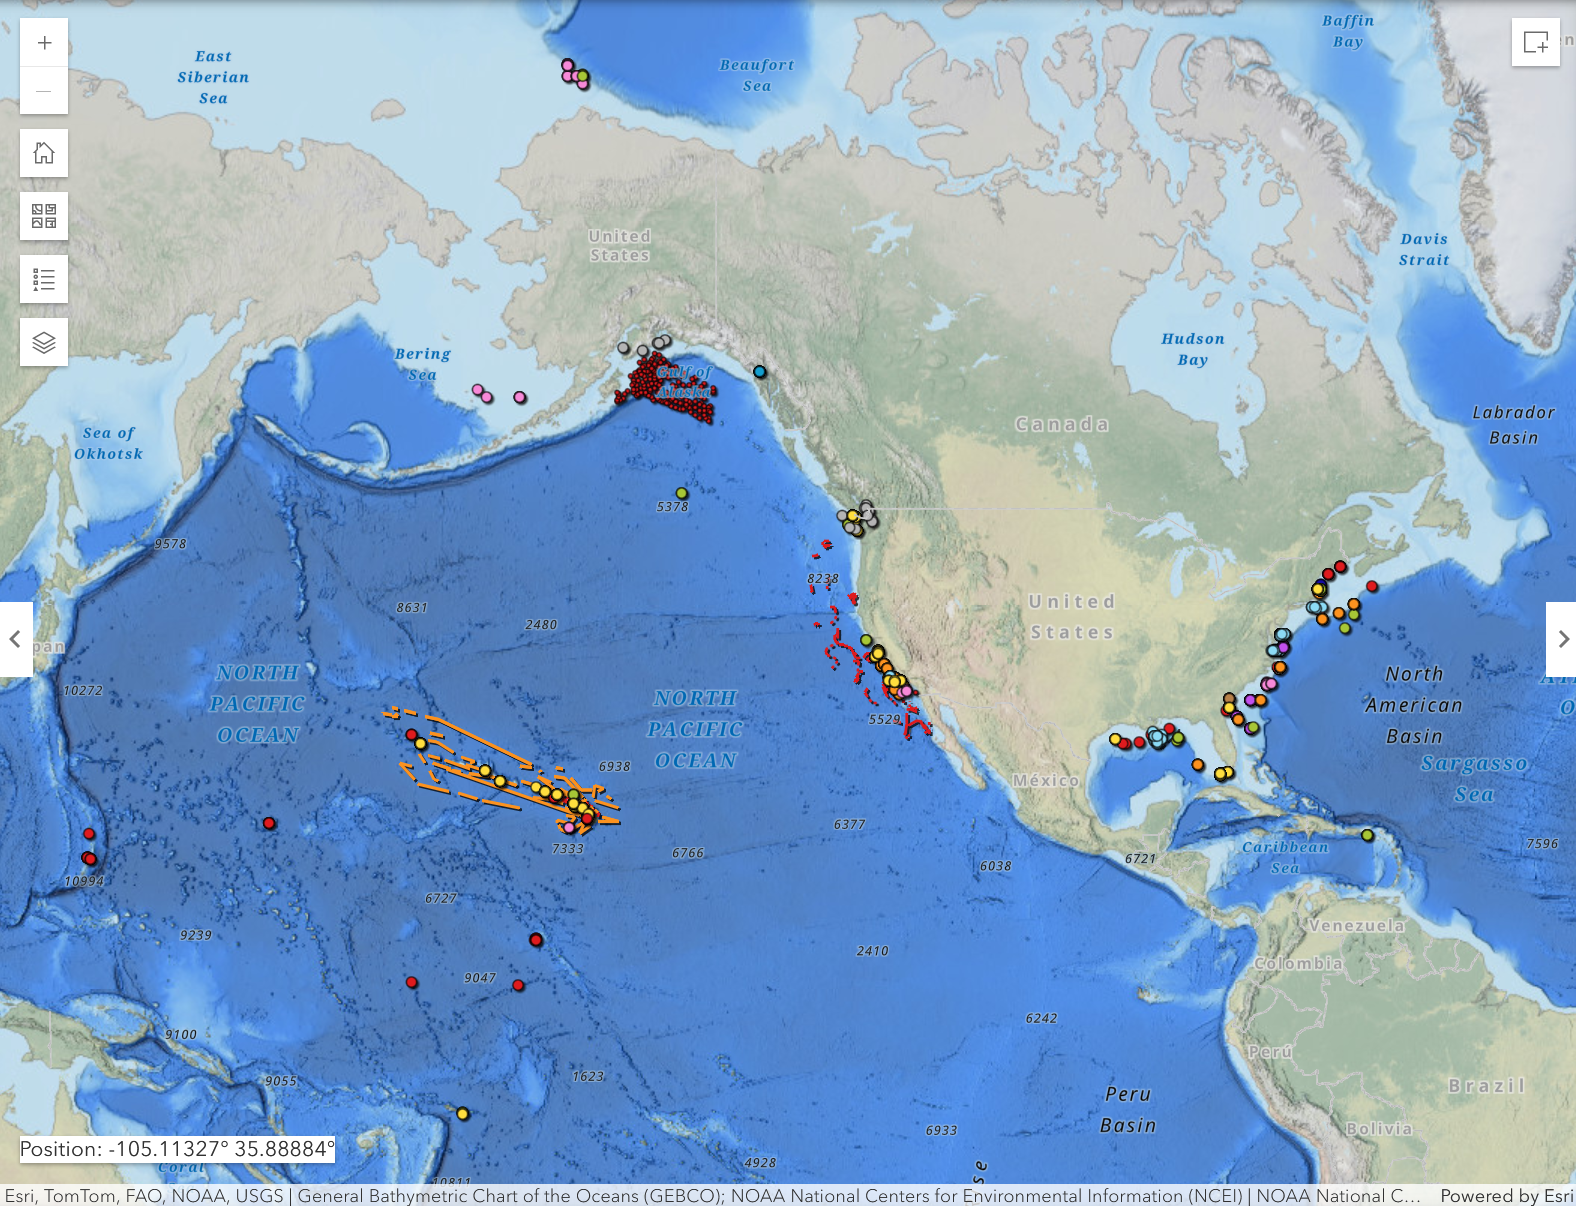
\includegraphics[height=0.4\textheight,width=0.7\textwidth,keepaspectratio]{images/aid_1.jpg}
    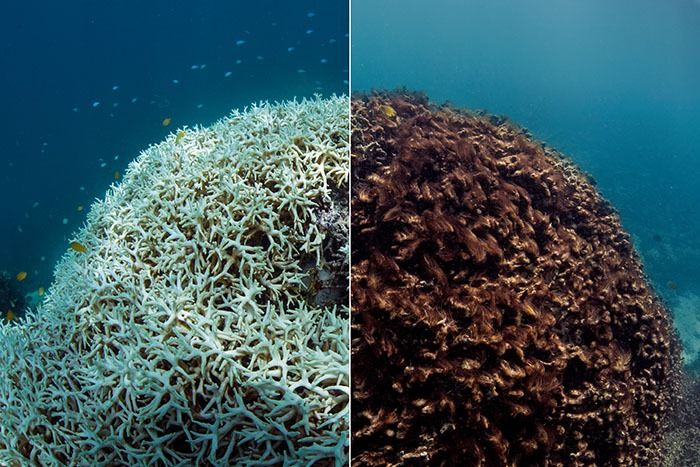
\includegraphics[height=0.4\textheight,width=0.7\textwidth,keepaspectratio]{images/aid_2.jpg}
\end{frame}

\begin{frame}{Vector Databases}
    
\end{frame}

\begin{frame}{Binary Classifier}
    
\end{frame}

\begin{frame}{Collar Team Agenda}
    \begin{itemize}
        \item Environment Configurations
        \item Integration Status
        \item Power Studies
    \end{itemize}
\end{frame}

\begin{frame}{Environment Configurations}
    \begin{itemize}
        \item CMSIS Library, BSP Package, and X-Cube-AI installations
        \item Individual environment setup configurations
        \item New Github repository for better organization
    \end{itemize}
\end{frame}

\begin{frame}{Integration Status}
    \begin{itemize}
        \item Slight delays in integration due to environment setup
        \item Work seperated into microphone, inference, and mel-spectrogram
        \item 
    \end{itemize}   
\end{frame}

\begin{frame}{Power Studies}
    \begin{itemize}
        \item Researching power optimization techniques
        \item Analyzing power consumption patterns
        \item Identifying opportunities for optimization
    \end{itemize}
\end{frame}

% To create a slide with a bullet list, use the following:
% \begin{frame}{TITLE}
%     \begin{itemize}
%         \item ITEM 1
%         \item ITEM 2
%     \end{itemize}    
% \end{frame}

% To create a slide with numbered list, use the following:
% \begin{frame}{TITLE}
%     \begin{enumerate}
%         \item ITEM 1
%         \item ITEM 2
%     \end{enumerate}
% \end{frame}

% To create a slide with a graphic:
% 1. Add the graphic to this folder (named picture.png)
% 2. Use the following:
% \begin{frame}{TITLE}
%     \centering
%     \includegraphics[height=0.7\textheight,width=0.7\textwidth,keepaspectratio]{picture.png}
% \end{frame}

% To create a slide with two columns, use the following:
% \begin{frame}{TITLE}
%     \begin{columns}
%         \begin{column}{0.5\textwidth}
%             COLUMN 1 BODY
%         \end{column}
%         \begin{column}{0.5\textwidth}
%             COLUMN 2 BODY
%         \end{column}
%     \end{columns}
% \end{frame}
